%----------------------------------------------------------------------------------------
%
% LaTeX-template for degree projects at LNU, Department of Computer Science
% Last updated by Johan Hagelbäck, Oct 2015
% Linnaeus University
%
% License: Creative Commons BY
%
%----------------------------------------------------------------------------------------

%----------------------------------------------------------------------------------------
%	Settings and configuration
%----------------------------------------------------------------------------------------

\documentclass[a4paper,12pt]{article}

\usepackage[T1]{fontenc}
\usepackage{times}
\usepackage[english]{babel}
\usepackage[utf8]{inputenc}
\usepackage{wallpaper}
\usepackage[absolute]{textpos}
\usepackage[top=2cm, bottom=2.5cm, left=3cm, right=3cm]{geometry}
\usepackage{appendix}
\usepackage[nottoc]{tocbibind}
\usepackage{enumerate}
\usepackage{array}
\newcolumntype{L}[1]{>{\raggedright\let\newline\\\arraybackslash\hspace{0pt}}m{#1}}

\setcounter{secnumdepth}{3}
\setcounter{tocdepth}{3}

\usepackage{sectsty}
\sectionfont{\fontsize{14}{15}\selectfont}
\subsectionfont{\fontsize{12}{15}\selectfont}
\subsubsectionfont{\fontsize{12}{15}\selectfont}
\usepackage[font=large, labelfont=bf]{caption}

\usepackage{csquotes} % Used to handle citations

\renewcommand{\thetable}{\arabic{section}.\arabic{table}}  
\renewcommand{\thefigure}{\arabic{section}.\arabic{figure}} 

%----------------------------------------------------------------------------------------
%	
%----------------------------------------------------------------------------------------
\newsavebox{\mybox}
\newlength{\mydepth}
\newlength{\myheight}

\newenvironment{sidebar}%
{\begin{lrbox}{\mybox}\begin{minipage}{\textwidth}}%
{\end{minipage}\end{lrbox}%
 \settodepth{\mydepth}{\usebox{\mybox}}%
 \settoheight{\myheight}{\usebox{\mybox}}%
 \addtolength{\myheight}{\mydepth}%
 \noindent\makebox[0pt]{\hspace{-20pt}\rule[-\mydepth]{1pt}{\myheight}}%
 \usebox{\mybox}}

%----------------------------------------------------------------------------------------
%	Title section
%----------------------------------------------------------------------------------------
\newcommand\BackgroundPic{
    \put(-2,-3){
    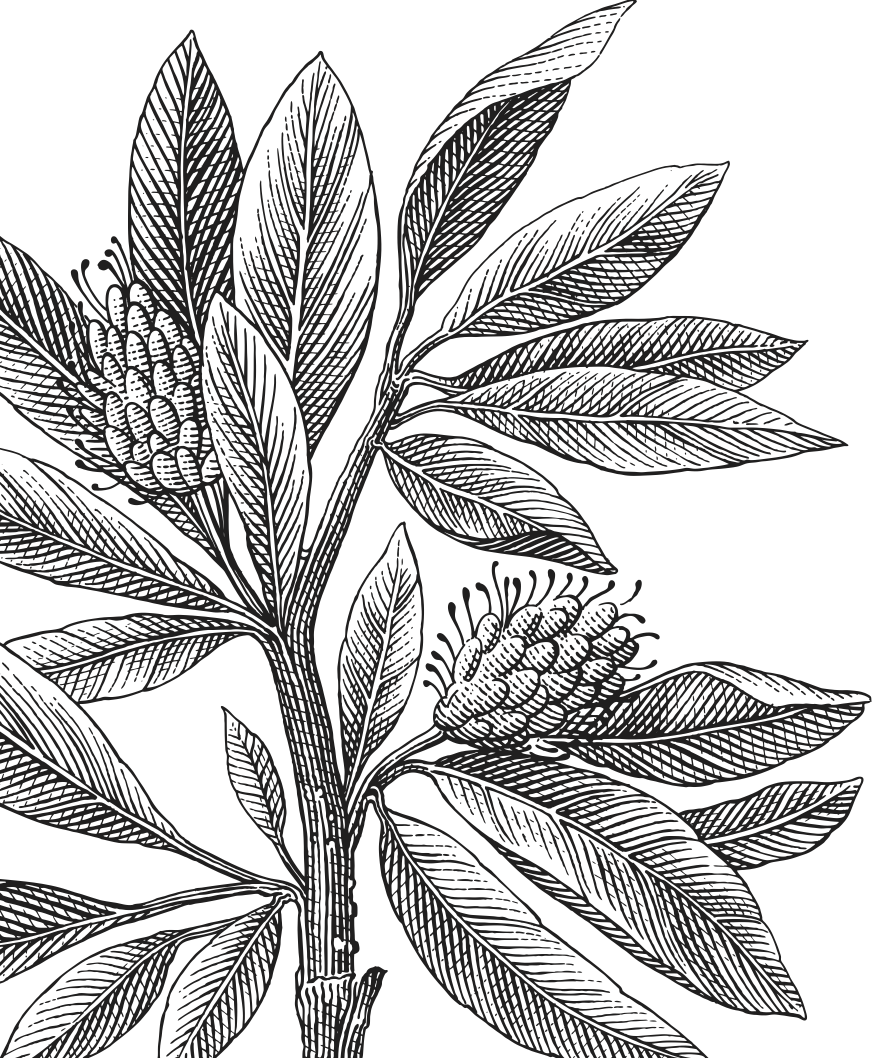
\includegraphics[keepaspectratio,scale=0.3]{img/lnu_etch.png} % Background picture
    }
}
\newcommand\BackgroundPicLogo{
    \put(30,740){
    
\includegraphics[keepaspectratio,scale=0.10]{img/logo.png} % Logo in upper left corner
    }
}

\title{	
\vspace{-8cm}
\begin{sidebar}
    \vspace{10cm}
    \normalfont \normalsize
    \Huge Report \\
    \vspace{-1.3cm}
\end{sidebar}
\vspace{3cm}
\begin{flushleft}
    \huge Project Course In Computer Science\\ 
    \it \LARGE - Deliveries Document
\end{flushleft}
\null
\vfill
\begin{textblock}{6}(10,13)
\begin{flushright}
\begin{minipage}{\textwidth}
\begin{flushleft} \large
\emph{Author:} Quasim Aljubarah, Michael Johansson, Tadas Lisauskas, Zeyuan Li, Robin Reijo and Robin Stempa\\ % Author
\emph{Supervisor:} Ola Petersson\\ % Supervisor
%\emph{Examiner:} Dr.~Mark \textsc{Brown}\\ % Examiner (course manager)
\emph{Semester:} VT 2016\\ % 
\emph{Subject:} 1DV508\\ % Subject area
\end{flushleft}
\end{minipage}
\end{flushright}
\end{textblock}
}

\date{} 

\begin{document}
\pagenumbering{gobble}
\newgeometry{left=5cm}
\AddToShipoutPicture*{\BackgroundPic}
\AddToShipoutPicture*{\BackgroundPicLogo}
\maketitle
\restoregeometry
\clearpage

\selectlanguage{english}



\newpage
\pagenumbering{gobble}
\pagenumbering{arabic}

%----------------------------------------------------------------------------------------
%
%	Here follows the actual text contents of the report.
%
%----------------------------------------------------------------------------------------
\section{Revision History}

\begin{table}[htbp]
	\centering
	\begin{tabular}{|L{4cm}|L{8cm}|L{4cm}|}
		\hline
		\textbf{Change} & \textbf{Description} & \textbf{Name and Date} \\ \hline
		Created Revision history table	&       included a revision history table to the document           &     Michael Johansson, 18/4 -2016               \\ \hline
	Updated status	&  Updated status on the deliveries for the first implementations seminar             &        Michael Johansson 19/4 -2016                \\ \hline
	Updated status &	Updated delivery 1 and 2	&	Michael Johansson 26/4 - 2016  \\ \hline
	Updated status & Updated delivery 3		& Michael Johansson 3/5 - 2016		\\ \hline
	Updated status & Updated delivery 4 and moved forward undone stuff from delivery 3 & Michael Johansson 10/5 - 2016 \\ \hline
	Updated some IDs & Updated the last IDs and change some text & Michael Johansson 30/5 - 2016 \\ \hline
	& & \\ \hline
	\end{tabular}
\end{table}
\newpage

\begin{table}[htbp]
	\centering
	\caption{Deliveries}
	\label{my-label}
	\begin{tabular}{|L{4cm}|L{7cm}|L{4cm}|}
		\hline
		\textbf{Delivery and Date}& \textbf{Description and IDs}                                                                                                                                                                                                                                                                                   & \textbf{Status} \\ \hline
		\textbf{Delivery 1  20/4 - 2016} & The admin page functionality should be almost done with add product etc. \newline The database should be up and running with all the tables done and all columns. \newline IDs to be done: 1, 1.1, 1.2, 1.3, 3, 3.1, 3.2                                                                  &     Admin page: Done \newline Edit product: Small delay \newline Database: done exept inserted all categories            \\ \hline
		\textbf{Delivery 2 27/4 - 2016} & The admin should be able to add, replace and remove categories. \newline All the categories should be defined. \newline IDs to be done: 1.1.2, 3.2.3, 3.2.4                                                                                                                                            &  Categories started and some is defined in the database  delayed           \\ \hline
		\textbf{Delivery 3 4/5 - 2016}  & The Cart should be working so the User can add, remove and change products in the cart. \newline IDs to be done: 2.2, 2.2.1, 2.2.2, 2.2.3                                                                                                                                                      &  Cart: Done \newline Categories still delayed                \\ \hline
		\textbf{Delivery 4 11/5 - 2016} & The User should be able to search, show all products in category and browse all products. \newline Admin should be able to add new and remove existing admin accounts. \newline The admin should be able to create new categories and edit/remove them. \newline IDs to be done: 2, 2.1, 3.3, 3.3.1          &  The User can search for products but not for categories. \newline Product page is \underline{not} done. \newline Admin can edit and add new admin accounts. \newline Admin can \underline{not} update categories or add new categories.              \\ \hline
		\textbf{Delivery 5 18/5 - 2016} & The User should be able to place orders.\newline The User should get an orderID when placing an order. \newline The User should be able to check his order with the orderID. \newline The User should be able to click on a product to get more info about it. \newline The admin should be able to create new categories.\newline IDs to be done: 1.2, 1.2.1, 2.3, 2.3.1, 2.3.2, 2.3.3, 3.2.3, 3.2.4, 3.4, 3.4.1 & User can place orders. \newline Users get a order ID and can check the order. \newline We can click on product names and get to the specific product page. \newline Admins can create new Categories.            \\ \hline
		\textbf{Delivery 6 25/5 - 2016} &  An Admin should be able to change and update orders. \newline The admin should be able to create new categories and edit/remove categories \newline IDs to be done: 3.2.3, 3.2.4, 3.4, 3.4.1, 3.4.2 & Admin can now edit orders, add new categories and edit categories.                   \\ \hline
		Delivery LATE &  CSS fine tune. \newline 		&		\\ \hline
	\end{tabular}
\end{table}
\end{document}
